\documentclass{article}
\usepackage{graphicx}
\graphicspath{ {./Figures/config1/} }
\begin{document}


\section{Initial model}

In this model, we have three populations: "go," "grow," and "gone." They each
have the same birthrate and same deathrate. Additionally, go can change into
grow, and grow and change into gone. The idea is to have two epithelial cell
types (go and grow) and one endothelial cell type (gone). Perastalsis is not
implemented in this model.

\subsection{Semi-arbitrary parameter simulation}

birthRate = 1.15

deathRate = 1

growToGoRate = 0.1

goToGoneRate = 0.1

startingGrow = 100

startingGo = 0

startingGone = 0

duration = 8

totalSimulations = 10000

dataPoints = 100

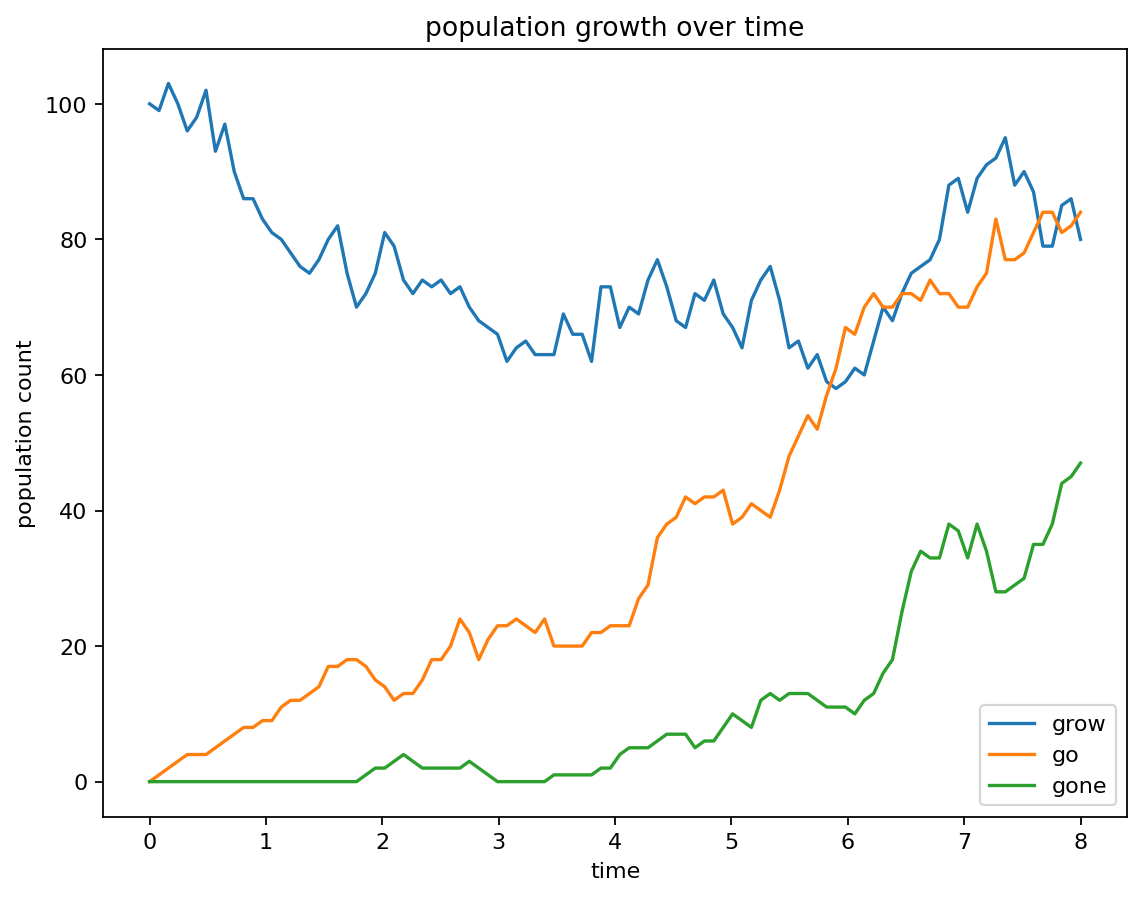
\includegraphics[width = 4in]{sim1.png}

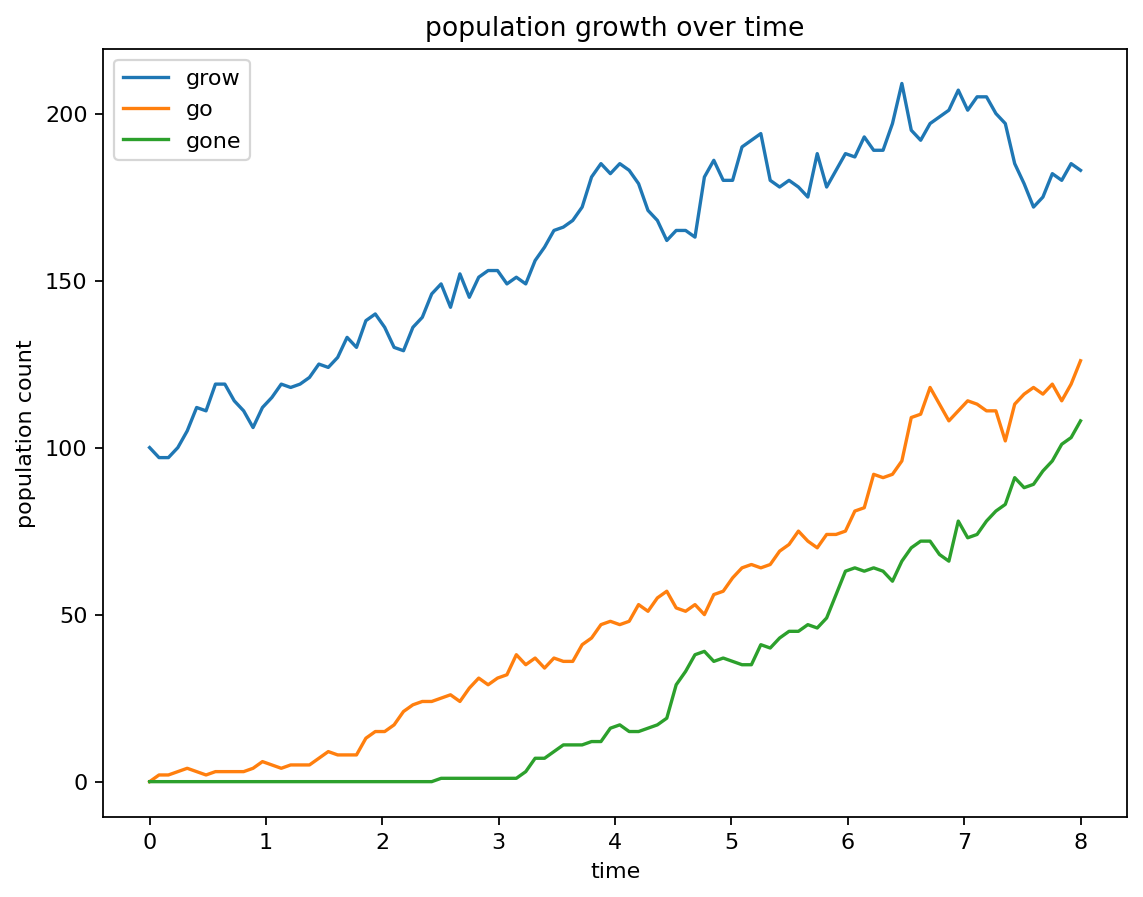
\includegraphics[width = 4in]{sim2.png}

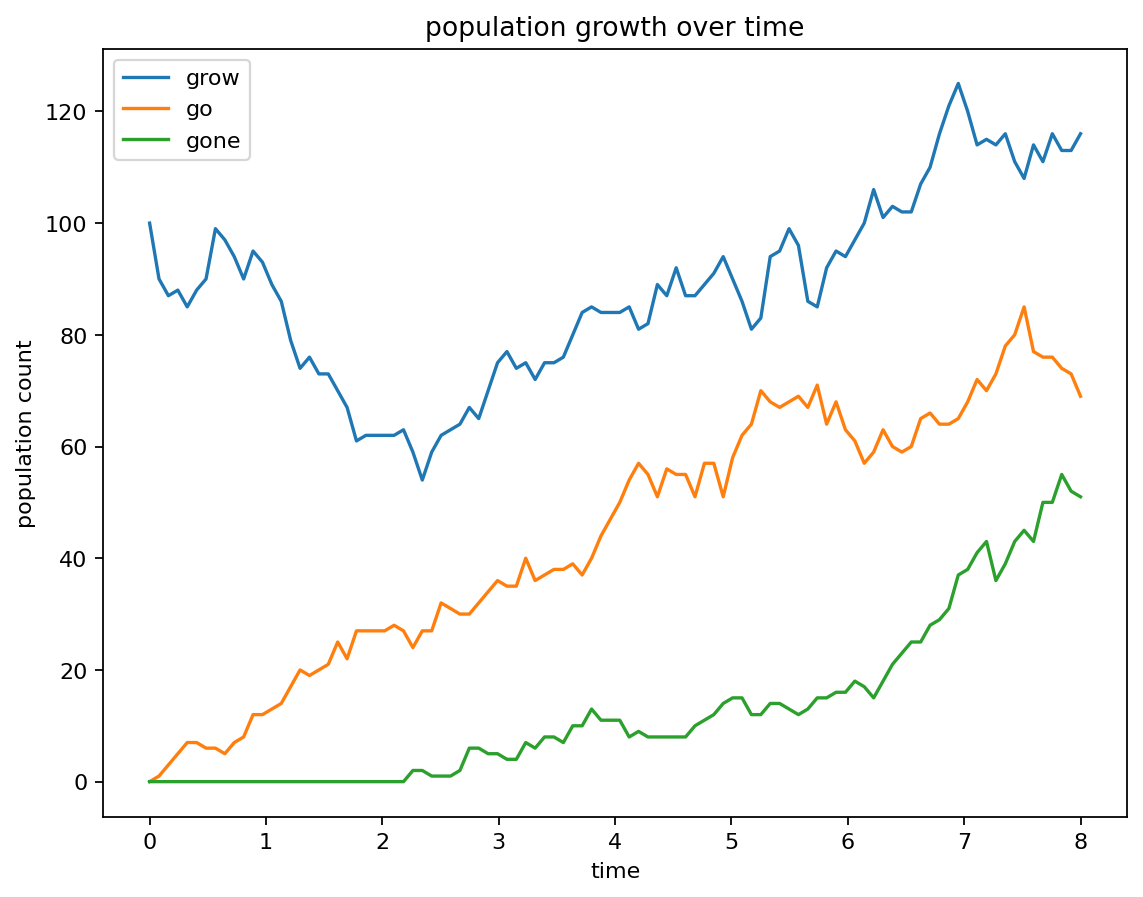
\includegraphics[width = 4in]{sim3.png}

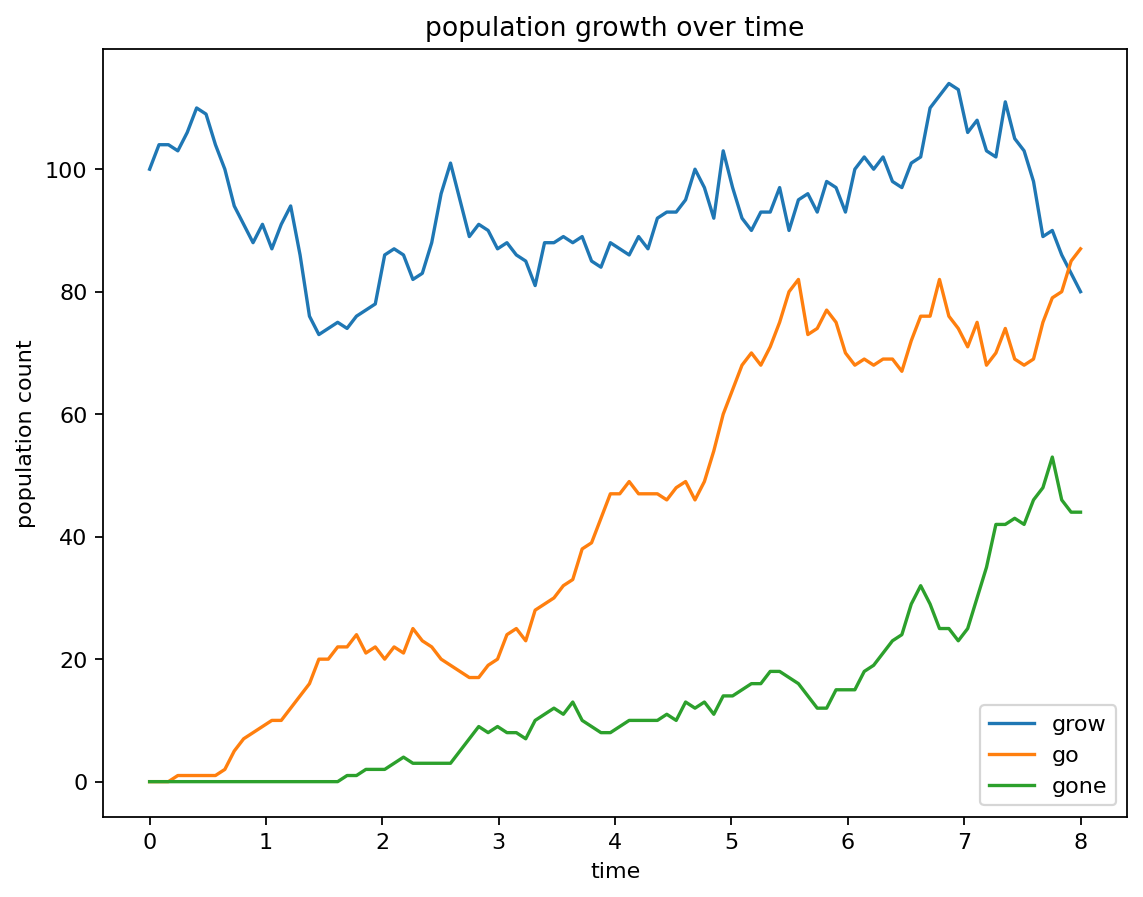
\includegraphics[width = 4in]{sim4.png}

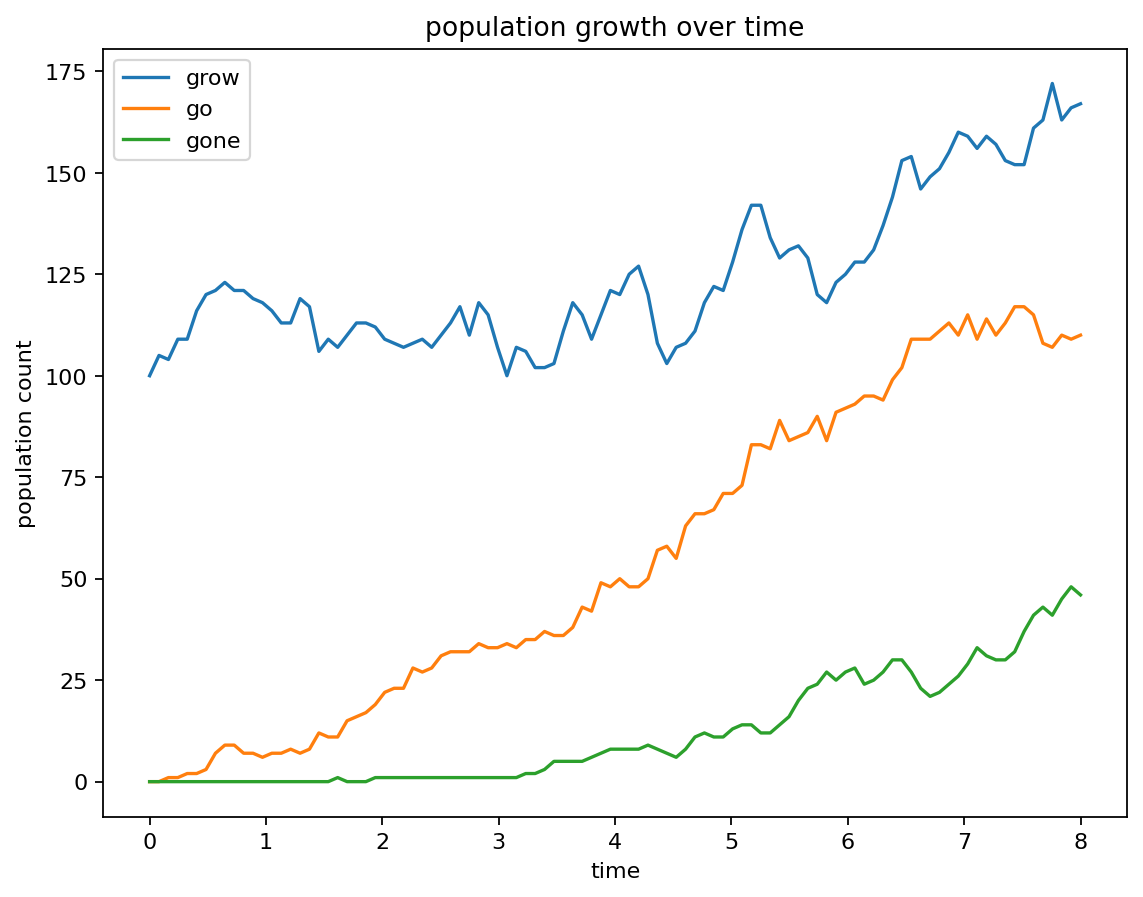
\includegraphics[width = 4in]{sim5.png}

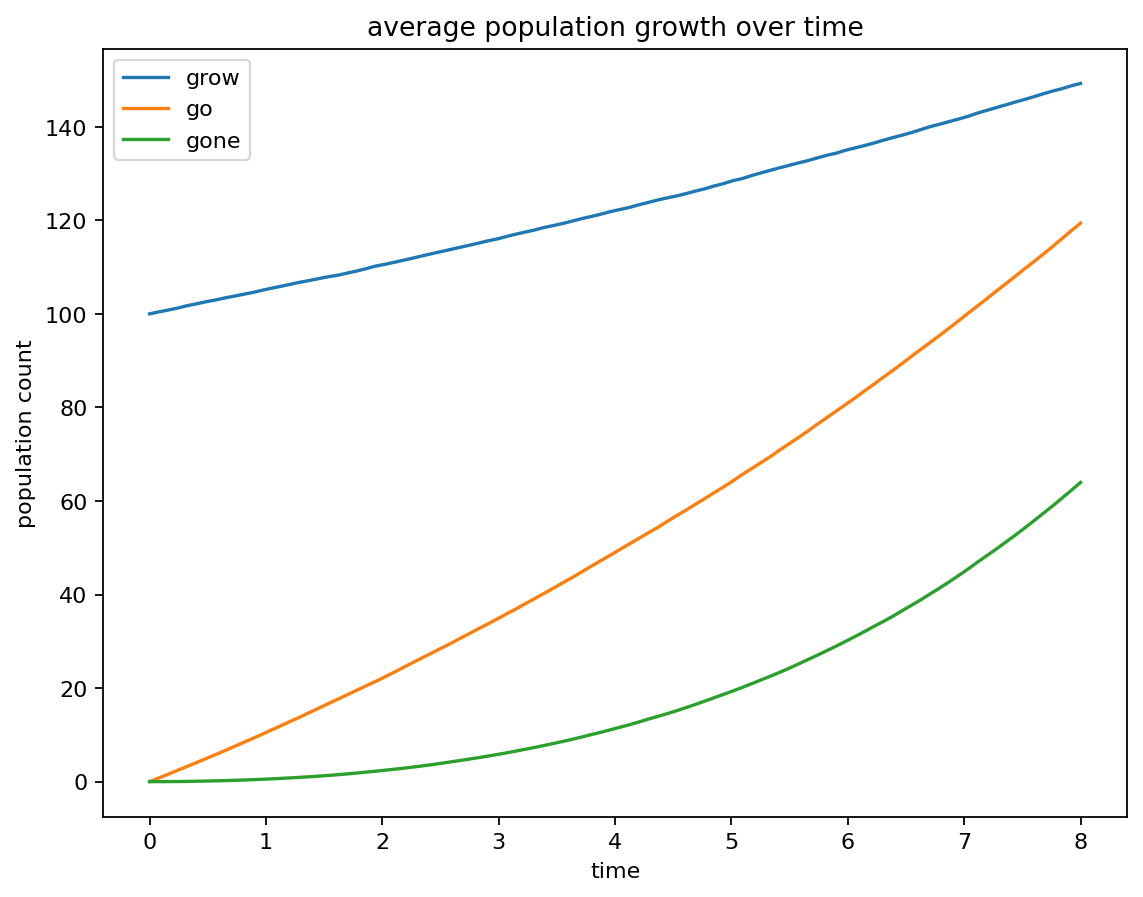
\includegraphics[width = 4in]{simMean.png}

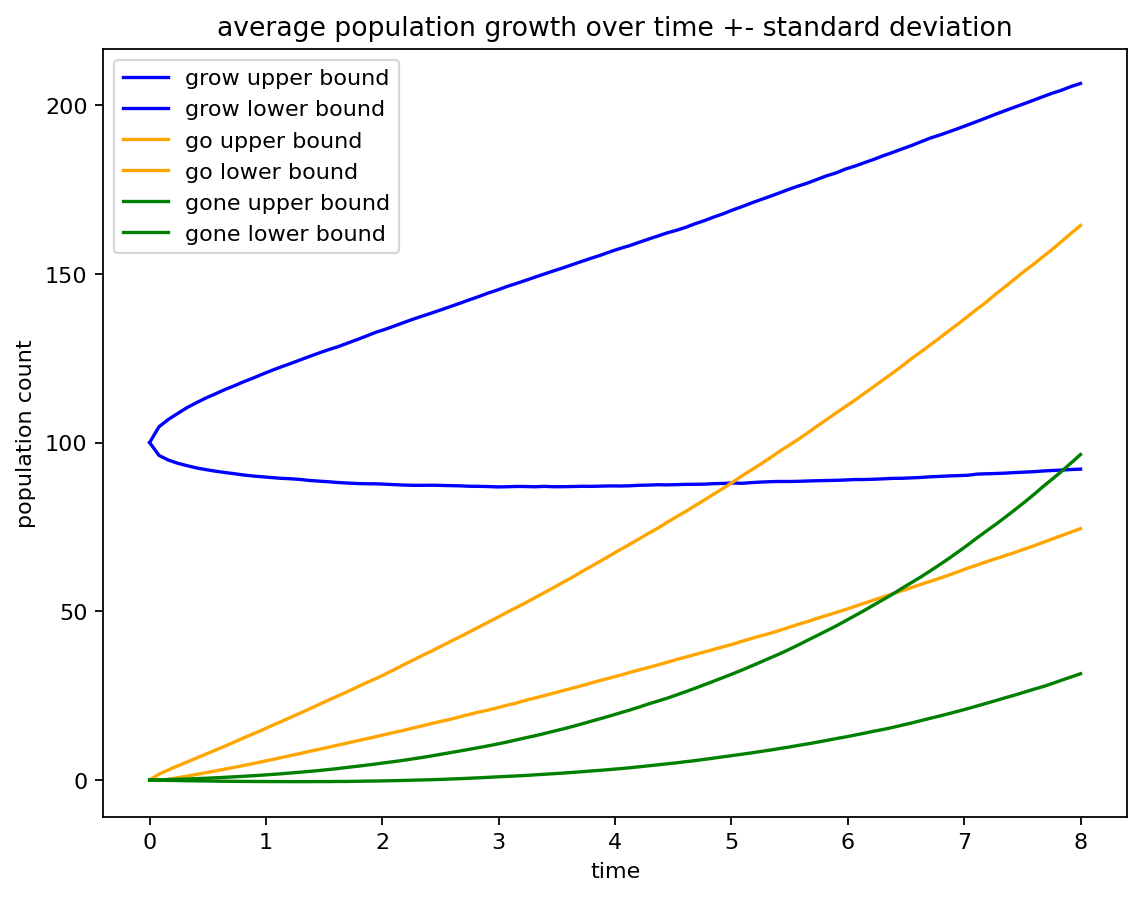
\includegraphics[width = 4in]{simBounds.png}
\end{document}
